
%% \textbf{@Pooyan,Andrea: here we should probably elaborate on OSTIA's architecture and the design principles that led us to define it as such... also we might want to elaborate on its components, the structure I'm suggesting below is merely tentative but it will give us ahead start!!}

%% \begin{itemize}
%% \item add and comment the meta-model of storm and how OSTIA uses that as a reference to draw and check models which are consistent with the technology
%% \item OSTIA Architecture
%% \item we should probably elaborate the architecture part (or on a separate "implementation" part or paragraph) with a link to the downloadable technology - @Andrea: can we bundle it up as plugin for Eclipse? E.g., somehow using RCP?
%% \item OSTIA Antipatterns Module
%% \item OSTIA Visualisation Module
%% \item OSTIA extensibility
%% \item OSTIA explanation of use and simple usage scenario
%% \item OSTIA explanation of use and simple usage scenario of continuous architecting
%% \end{itemize}
This section outlines OSTIA starting form a brief recap of the technology it is currently designed to support. Further on, the section introduces how OSTIA was designed to support design-time analysis and continuous improvement of data-intensive applications, using the case of streaming topologies in Storm as a running example. Finally, the section outlines an example meta-model for Storm that captures all restrictions and rules (e.g., for configuration, topology, dependence, messaging, etc.) in the framework. OSTIA uses this and similar meta-models as a reference every time the application is run to recover and analyse operational topologies.

\subsection{OSTIA Tool Architecture}

The overall architecture of OSTIA is depicted in
Figure \ref{archostia}. The logical architectural information of the
topology is retrieved by OSTIA via static analysis of the source code. OSTIA
generates a simple intermediate format to be used by other algorithmic
processes.

OSTIA is architected in a way that additional algorithmic analyses similar to our anti-pattern
analyses can be easily added. These analyses use the information resides in the
intermediate format and provide added value analyses for design-time analysis and verification. Since the information in the intermediate format only rely
on the logical code analysis, the algorithmic analyses require some
information regarding the running topology, such as end to end latency and
throughput.

\begin{figure}[H]
	\begin{center}
		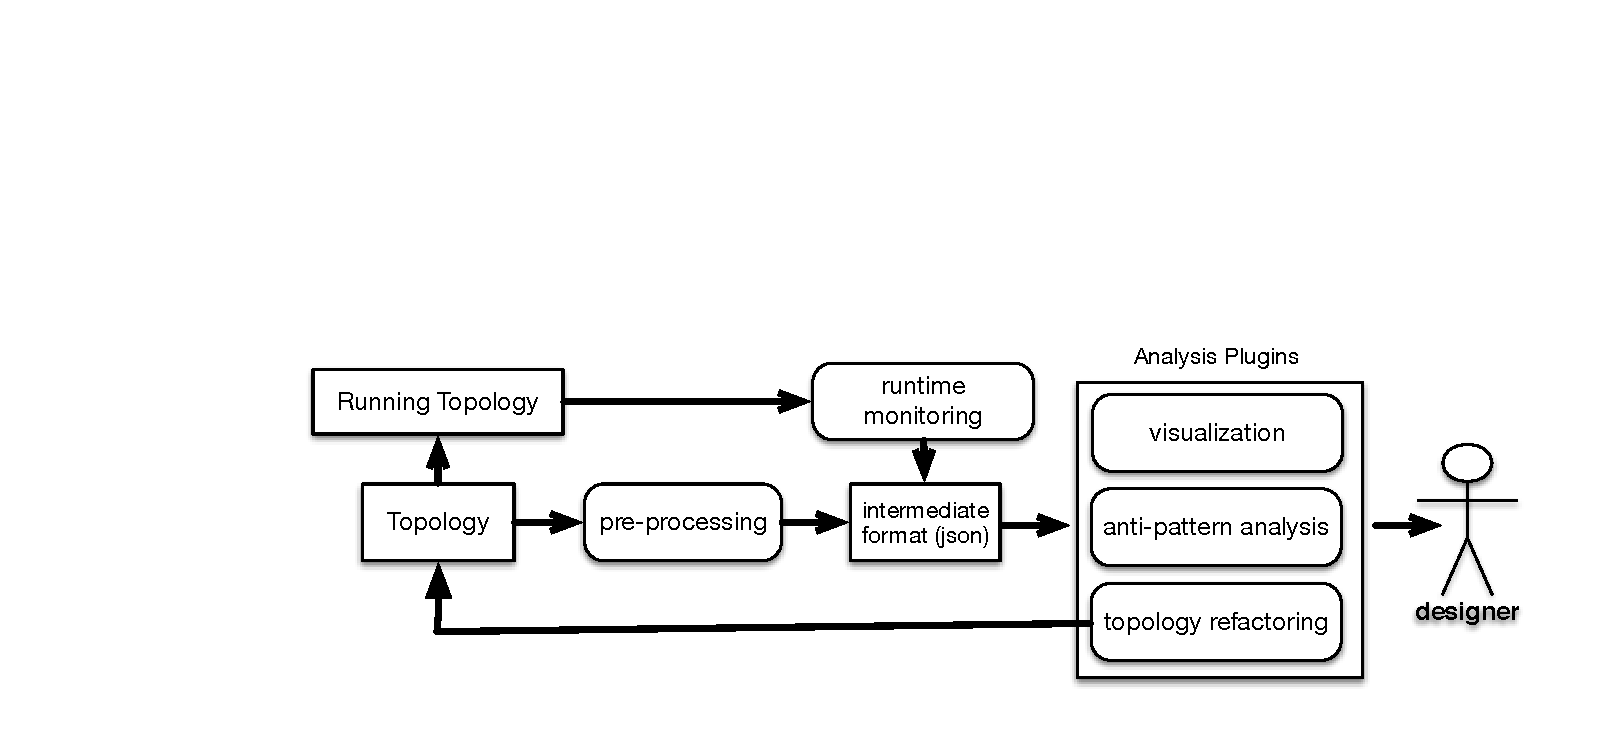
\includegraphics[width=9cm]{images/ostia-arch}
		\caption{OSTIA extensible architecture.}\label{archostia}
	\end{center}
\end{figure}

Such information will be continuously added to the intermediate repository via
runtime monitoring of the topology on real deployment cluster. These provide
appropriate and rich information for refactoring the initial architecture and
enabling performance-driven DevOps \cite{brunnert2015performance}.
Finally, OSTIA allows users to export the topology in different formats
(specifically, JSON, Dot, CSV, and XMI) to analyse and continuously improve the topology with other tools --- in the scope of this paper we focus on verification \emph{by-design} featuring formal verification.

%%%\subsection{A Concrete Example: The Storm Architecture}
%%%
%%%Storm is a technology developed at Twitter \cite{toshniwal2014storm} in order to
%%%face the problem of processing of streaming of data. It is defined as a
%%%distributed processing framework which is able to analyse streams of data. A Storm topology is a computational graph composed by nodes of two types: spouts and bolts. The former type includes nodes that process the data entering the topology, for instance
%%%querying APIs or retrieve information from a message broker, such as Apache
%%%Kafka\footnote{\url{http://kafka.apache.org/}}. The latter executes operations on data, such as filtering or serialising.
%%%
%%%\subsubsection{Storm Framework Meta-Model}
%%%
%%%OSTIA was designed to retrieve and analyse big data topologies, allowing their refactoring in a way which is consistent with framework restrictions, rules and regulations part of the Storm framework. To do so, OSTIA uses a meta-model for the Storm framework which acts as an operational image of all said restrictions and rules that OSTIA needs to maintain. 
%%%Essentially OSTIA uses the meta-model as such an operational image for Storm, for two purposes: (a) checking that Storm restrictions (e.g., Spouts initiate the topology) and constraints (e.g., grouping policies) are valid on models recovered by OSTIA; (b) keep checking said restrictions and constraints during continuous architecting. \todoMB{}{Chiarire.}
%%%To give a hint of the complexity of the technology, we outline the meta-model in Fig. \ref{stormmm}. where, for example, the grouping restrictions that Storm envisions are captured in an enumeration of constraints (see the $<<$Grouping$>>$ element or the $<<$ReplicationFactor$>>$ concrete parameter). Key elements of the meta-model are the following:
%%%\begin{itemize}
%%%\item $<<$TopologyConfiguration$>>$ contains the parameters necessary for the Storm framework to be configured and to run on the selected infrastructure. OSTIA checks that these parameters are present or that defaults are correctly inplace;\todoMB{}{In che senso?}
%%%\item $<<$Topology$>>$ specifies the topological construct being elicited for the analysed Storm application, as composed of the $<<$Bolt$>>$ and  the $<<$Spout$>>$ meta-elements;
%%%\item  $<<$Grouping$>>$ contains restrictions on the possible groupings of the $<<$Bolt$>>$ and the $<<$Spout$>>$ meta-elements within the elicited topology. OSTIA checks these restrictions upon recovery and exporting of topologies;\todoMB{}{In che senso?}
%%%\end{itemize}
%%%
%%%\begin{figure*}
%%%\centering
%%%%	\begin{sideways}
%%%		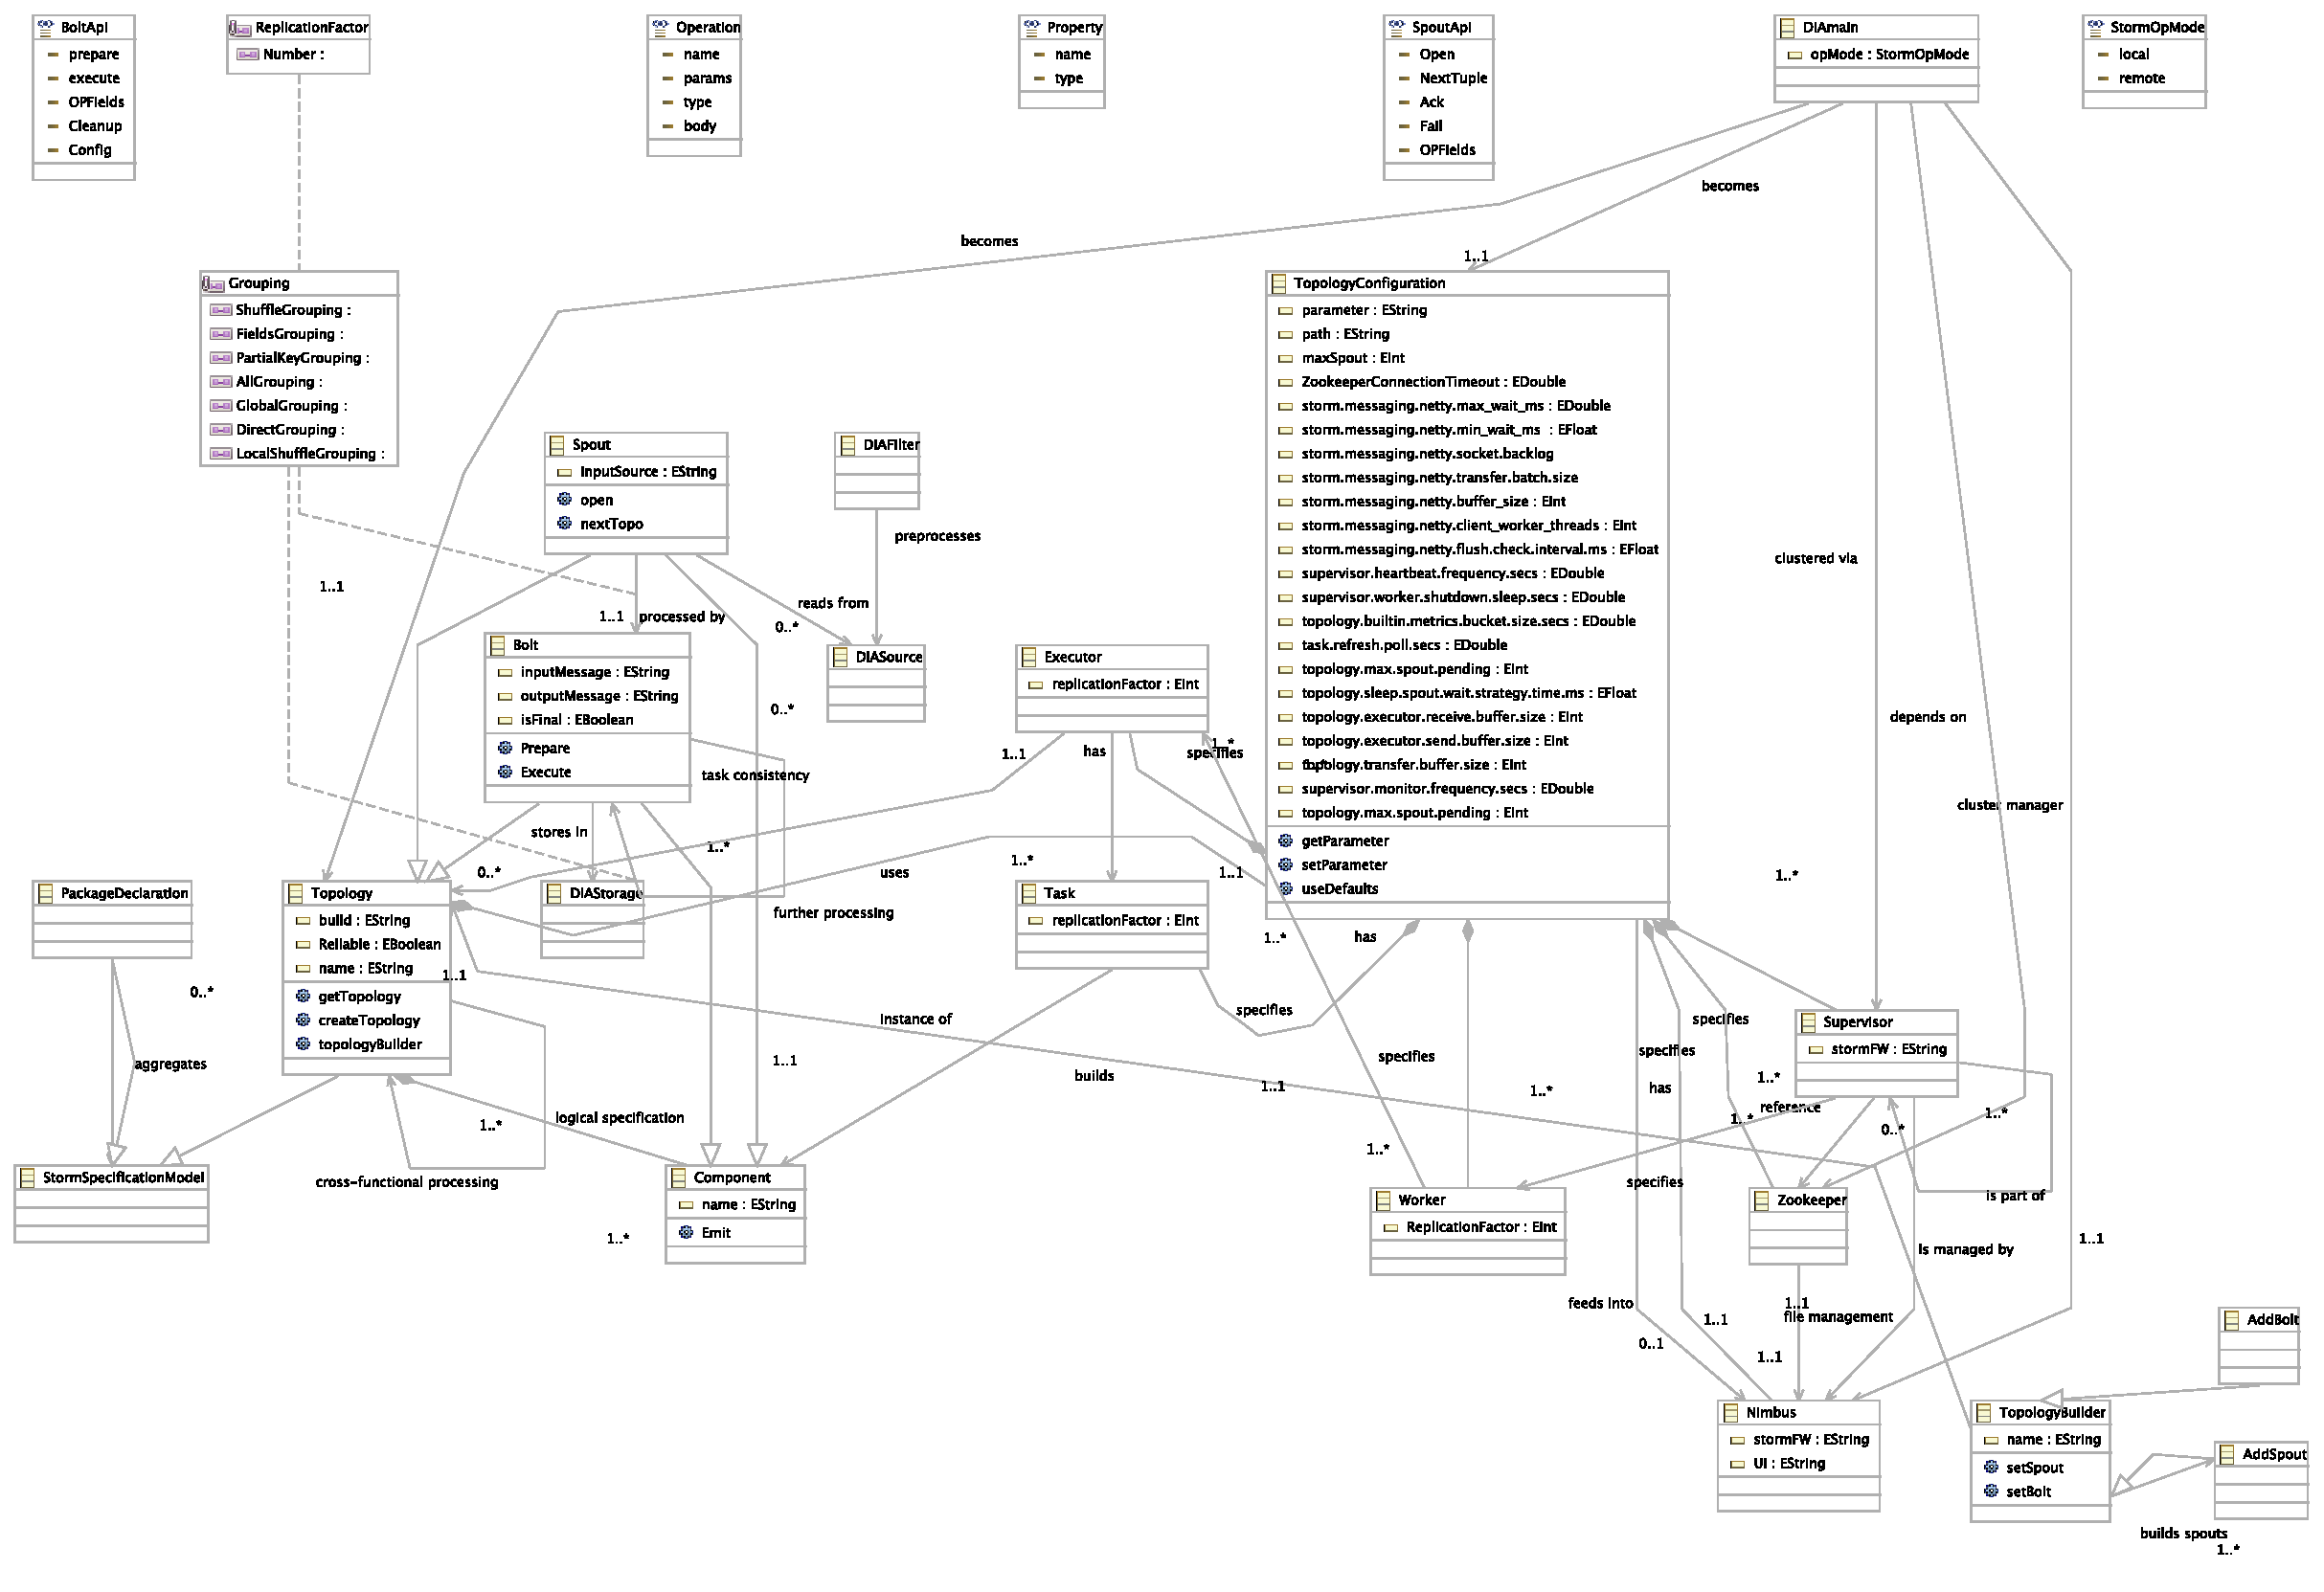
\includegraphics[width=16cm]{images/Stormmm}
%%%%	\end{sideways}
%%%	\caption{The Storm Meta-Model, an overview.}
%%%		\label{stormmm}
%%%\end{figure*}
%%%
%%%A complete overview of the details of this meta-model and the restrictions captured therein is beyond the scope of this paper - rather, the entire purpose of OSTIA is to hide their complexity: for example, notice the \emph{TopologyConfiguration} meta-class, where we deliberately selected 22 (about 10\% of the entire set) of parameters possibly configurable for running Storm topologies. Further detail on the Storm meta-model may be found on the full technical report describing our technology\footnote{\url{http://dice-h2020.eu/deliverables/D2.1}}.
%%%%\comment{a description about the verification analyses and more details about the implementations should be added here}
%%%
%%%\subsubsection{Storm: A Formal Interpretation}
%%%Model-checking can serve as a means to enact continuous architecting of Storm topologies. Topologies can undergo formal verification, for example, to assess temporal properties on their execution.
%%%This section elaborates on the role of formal verification in OSTIA and describes the necessary background, modelling assumptions and model definition behind Storm topology verification.
%%%In particular, we provide a non-deterministic model representing Storm topologies' behavior in terms of the delay connected to bolts' processing, spout input profile and node failures. Spout input profile is measured with rates of incoming tuples into the topology.
%%%Verification in OSTIA is intended to discover possible design errors at design time which are caused by (i) under/over estimation of timing requirements of computational nodes or (ii) possible runtime node failures.
%%%Therefore, in this context, we are interested in verifying properties like, for instance, the existence of an execution of the topology which guarantees queue-length boundedness even if failures occur with a certain delay.
%%%Defining the formal model, requires the comprehension of %started by understanding and capturing 
%%%the behaviors of both spouts and bolts which, after choosing the level of abstraction of the model, allows us to abstract those behaviors accordingly, %in order 
%%%to formalize them as finite state machines. The purpose of this activity is defining the %possible 
%%%operations performed by nodes and their allowed orderings in a real implementation. %of such operations.
%%%We then extend the model %by taking into account 
%%%considering the message buffers (or queues) and the quantity of tuples that are exchanged through the topology.
%%%In addition, %to the correct ordering of the operations, we decided to 
%%%we introduce more specific temporal constraints %into the model, in order 
%%%to limit the time spent by the system in each state (or processing phase) and to elaborate the concept of \textit{rate}, intended as ``number of times an event is occurring every time unit''.
%%%The formal modeling (see Section \ref{ver}) is based on real-time temporal logic, i.e., the topology behavior is defined through a temporal logic formula written in Constraint LTL over clocks (CLTLoc)~\cite{BRS15}.

